\documentclass[10pt,twoside,openright,a4paper]{report}

% Adds support for UTF-8 text
\usepackage[utf8]{inputenc}
% Margins will have 2.5cm
\usepackage[margin=2.5cm]{geometry}
% Used for line spacing
\usepackage{setspace}
% Adds support for referencing
\usepackage{hyperref}
% Fixes references to footnotes
\usepackage[all]{hypcap}
% Support for colors in tables
\usepackage{booktabs}
\usepackage[table,xcdraw]{xcolor}
% Adds support for figures
\usepackage{graphicx}
% Adds support for helvetica font
\usepackage{helvet}
% Uses the portuguese and english dictionaries
\usepackage[portuguese,english]{babel}
% Adds support for acronyms and to generate the table of contents
\usepackage[acronym, toc]{glossaries}
% Allows to import pdf pages
\usepackage{pdfpages}
% Adds support for source code listing
\usepackage{listings}
\lstset{language=Matlab}
% Allows underlined sentences to break when reaching EOL
\usepackage{soul}
% Allows the creation of colors to use along the document
%\usepackage{color}
% Adds support for source code listing with colors
%\usepackage{minted}
% Adds support for inline itemize
\usepackage[inline]{enumitem}
% Adds support for multiple line equations
\usepackage{amsmath}
% Adds support for captions
\usepackage{caption}
% Indent First Line of Chapter
\usepackage{indentfirst}
% Adds support for multiple rows in a table
\usepackage{multirow}
% Allow usage of statistical symbols
\usepackage{amssymb}

% Builds the glossary when the main file is built.
\makeglossaries
% Set main font to Arial
\renewcommand{\familydefault}{\sfdefault}
% Define keywords macro
\providecommand{\keywords}[1]{\textbf{Keywords:} #1}
\providecommand{\palavraschave}[1]{\textbf{Palavras-chave:} #1}
% Define the NewPage macro
\newcommand*\NewPage{\newpage\null\thispagestyle{empty}\cleardoublepage}
% Abstract-en page numbering
\newcommand {\abstractEnglishPageNumber} {\thispagestyle{plain}\setcounter{page}{\abstractEnglishPage}}
% Abstract-pt page numbering
\newcommand {\abstractPortuguesePageNumber} {\thispagestyle{plain}\setcounter{page}{\abstractPortuguesePage}}
% Section numbering depth
\setcounter{secnumdepth}{2}
% Table of contents depth
\setcounter{tocdepth}{3}
% Set line spacing to 1.5cm
\onehalfspacing
% Page numbering
\pagestyle{plain}

% Add acronyms
%!TEX root = ../article.tex

\newacronym{IST}{IST}{Instituto Superior T\'ecnico}
\newacronym[plural=EPEs,firstplural=Event Processing Engines (EPEs)]{EPE}{EPE}{Event Processing Engine}
\newacronym[plural=EPNs,firstplural=Event Processing Networks (EPNs)]{EPN}{EPN}{Event Processing Network}
\newacronym[plural=EPs,firstplural=Event Providers (EPs)]{EP}{EP}{Event Provider}
\newacronym[plural=EPAs,firstplural=Event Processing Agents (EPAs)]{EPA}{EPA}{Event Processing Agent}
\newacronym[plural=ECs,firstplural=Event Consumers (ECs)]{EC}{EC}{Event Consumer}
\newacronym[plural=DAGs,firstplural=Directed Acyclic Graphs (DAGs)]{DAG}{DAG}{Directed Acyclic Graph}
\newacronym{API}{API}{Application Programming Interface}
\newacronym{YAML}{YAML}{YAML Ain't Markup Language}
\newacronym{HTTP}{HTTP}{Hypertext Transfer Protocol}
\newacronym{REST}{REST}{Representational State Transfer}
\newacronym{JSON}{JSON}{JavaScript Object Notation}
\newacronym{URL}{URL}{Uniform Resource Locator}
\newacronym{IT}{IT}{Information Technology}
\newacronym{BPA}{BPA}{Business Process Automation}
\newacronym{RSS}{RSS}{Rich Site Summary}
\newacronym{SaaS}{SaaS}{Software as a Service}
\newacronym{XML}{XML}{eXtensible Markup Language}
\newacronym{DBMS}{DBMS}{Database Management Systems}
\newacronym{SOA}{SOA}{Service-oriented Architecture}
\newacronym{IFTTT}{IFTTT}{If This Then That}


% ------------------------------------------
% DISSERTATION
% ------------------------------------------

\begin{document}

% Set default programming language in source code listing to be Java
% \lstset{language=Java}

\pagenumbering{gobble}% Remove page numbers (and reset to 1)
\clearpage
\thispagestyle{empty}
%!TEX root = ./dissertation.tex

% Dissertation basic information
\newcommand {\Title} {Will It Blend?}
\newcommand {\StudentName} {Paulo Duarte Esperança Garcia}
\newcommand {\DegreeName} {Information Systems and Computer Engineering}
\newcommand {\MainSupervisor} {Prof. Dr. Daniel Jorge Viegas Gonçalves}
\newcommand {\SecondSupervisor} {Prof. Dra. Sandra Pereira Gama}
\newcommand {\Chairperson} {Prof. Dr. Someone}
\newcommand {\Advisor} {\MainSupervisor}
\newcommand {\CommitteeMembers} {Prof. Dr. Someone}

% Include or not include acknowledgments
\def \includeAcknowledgments{1}

% Date
\newcommand {\Month} {October}
\newcommand {\Year} {2016}

% Acknowledgments page number
\def \acknowledgmentsPage{1}

% Abstract-en page numbering
\def \abstractEnglishPage{3}

% Abstract-pt page number
\def \abstractPortuguesePage{5}

% You can define your own variables here
%\definecolor{name}{model}{color-spec}
\definecolor{red}{HTML}{FF0000}
\definecolor{green}{HTML}{00FF00}
\definecolor{blue}{HTML}{00FF00}


%!TEX root = ./dissertation.tex

% ---------------------------------------------------------
%   MASTER THESIS DISSERTATION COVER
% ---------------------------------------------------------
\begin{titlepage}
% ---------------------------------------------------------
%  INSTITUTION LOGO
% ---------------------------------------------------------

\includegraphics[width=5cm]{images/ist-logo}~\\[1.5cm]
\begin{center}
% ---------------------------------------------------------
%  MASTER THESIS DISSERTATION TITLE
% ---------------------------------------------------------
{\LARGE \textbf{\Title}}\\[1.5cm]
% ---------------------------------------------------------
%  AUTHOR NAME (FULL)
% ---------------------------------------------------------
{\Large \textbf{\StudentName}}\\[1.5cm]
% ---------------------------------------------------------
%  DISSERTATION DEGREE
% -----------------------------------------------------------------
{\large Thesis to obtain the Master of Science Degree in}\\[0.35cm]
% -----------------------------------------------------------------
%  COURSE NAME
% -----------------------------------------------------------------
{\LARGE \textbf{\DegreeName}}\\[1.5cm]

% -----------------------------------------------------------------
%  ADVISORS NAME
% ---------------------------------------------------------
\begin{minipage}[t]{.32\textwidth}
  \begin{flushright}
    {\large Supervisors:~~}\\
  \end{flushright}
\end{minipage}%
\begin{minipage}[t]{.68\textwidth}
  \begin{flushleft}
    {\large \MainSupervisor \\
     \large \SecondSupervisor}
  \end{flushleft}
\end{minipage}\\[1.5cm]

% ---------------------------------------------------------
%  JURI NAMES:
%  - PRESIDENT
%  - ADVISOR
%  - VOGALS
% ---------------------------------------------------------
{\Large \textbf{Examination Committee}}\\[0.75cm]

\begin{minipage}[t]{.4\textwidth}
  \begin{flushright}
    {\large Chairperson:\:}\\
    {\large Supervisor:\:}\\
    {\large Member of the Committee:\:}
  \end{flushright}
\end{minipage}%
\begin{minipage}[t]{.6\textwidth}
  \begin{flushleft}
    {\large \Chairperson}\\
    {\large \Advisor}\\
    {\large \CommitteeMembers}
  \end{flushleft}
\end{minipage}\\[6.5cm]

% ---------------------------------------------------------
%  DATE (MONTH AND YEAR)
% ---------------------------------------------------------
{\Large \textbf{\Month\:\Year}}\\
\end{center}
\end{titlepage}

\NewPage

\pagenumbering{roman}

\if\includeAcknowledgments 1
%!TEX root = ../dissertation.tex

\chapter*{Acknowledgments}
%
First, I want to thank my advisor Professor Daniel Gonçalves for his excellent guidance, of always having the availability to teach, help and
clarify, for his enormous knowledge and expertise, and for always believing in the best result possible of this Master Thesis. Then, I also
want to thank my co-advisor Sandra Gama, for her more-than-valuable inputs on Information Visualization and for opening the path for this
dissertation and others to come! \\ \par
%
Additionally, I would like to thank everyone which somehow contributed for this thesis to happen: everyone who participated either online,
or on the laboratory sessions, specially those who did it so willingly, without looking at the rewards. Without them, there would be no
validity is this thesis.  \\ \par
%
I must express my very profound gratitude to my family, particularly my mother Ondina and brother Diogo, for providing me with unfailing support
and continuous encouragement throughout my years of study and through the process of researching and writing this thesis. This accomplishment
would not have been possible without them. Thank you! \\ \par
%
Finally, to my girlfriend Margarida, my beloved partner, my shelter and support, for all the sleepless nights, sweat and tears throughout
the last seven years. Thank you for always believing in me, for being who you are, and for all the little things. \\

\NewPage
\fi

%!TEX root = ../dissertation.tex

\begin{otherlanguage}{english}
\begin{abstract}
\thispagestyle{plain}
\abstractEnglishPageNumber
Using color to convey information is not a recent rule: its usage is further associated to standards, statistics and computer
science. However, color is a subjective aspect of human perception, as it is strongly influenced by cultural background, childhood
learning and possible existent color vision deficiencies. Over the last years, research has been made to ascertain if color is the ideal
channel to transmit information; particularly, if the blending of two or more colors can convey, in a efficient way, the information
contained in two or more variables, using color blending techniques. \\
%
Nonetheless, previous investigation has not come to an agreement about to which extent can color blending techniques be used, in
an efficient and effective way, to convey information. \\
%
Our goal is to study if the users can detect the blending-basis when the result of a given color mixture is given, and vice-versa; moreover, it
is important to understand which color model has the best matching with the user's blending expectation, and detect colors which
may yield better results than others. \\
%
In order to achieve this, we have developed a user color study performed in an online and laboratory environment. This study was
based on a platform capable of gathering data from both environment, called \emph{BlendMe!}. Among other important details, this
user study was characterized by the creation of a color slider mechanism of presenting the user picked colors, whitout being
influenced by other unnecessary colors. \\
%
As product of this Master thesis, we intend to conclude relevant implications of using color blending techniques, in the Information
Visualization field of research. Additionaly, we will provide a set of questions apart from the ones answered by the us, which
remain unaswered and could be an interesting source of future work.
% Keywords
\begin{flushleft}

\keywords{colors, models, spaces, blending, InfoVis, color perception, user study, calibration, scales, organization, data
visulization, data processing, blending techniques, color vision deficiencies, demographic analysis}

\end{flushleft}

\end{abstract}
\end{otherlanguage}

\NewPage
%!TEX root = ../dissertation.tex

\begin{otherlanguage}{portuguese}
\begin{abstract}
\thispagestyle{plain}
\abstractPortuguesePageNumber
Resumo Português fica aqui.

% Keywords
\begin{flushleft}

\palavraschave{uma, duas, três, keywords}

\end{flushleft}

\end{abstract}
\end{otherlanguage}

\NewPage

% Table of contents
\tableofcontents
\cleardoublepage

% List of tables
\listoftables
\addcontentsline{toc}{chapter}{\listtablename}
\NewPage

% List of figures
\listoffigures
\addcontentsline{toc}{chapter}{\listfigurename}
\NewPage

% List of acronyms
\printglossary[type=\acronymtype]
\NewPage

\pagenumbering{arabic}% Arabic page numbers (and reset to 1)

% Chapters
%!TEX root = ../dissertation.tex

% Appendix chapters entry point
% Include the chapters below

%!TEX root = ../dissertation.tex

\chapter{User Study Protocol}
\label{appendix:protocol}

\section{Motivation}
%
By conducting this first study, we intend to:
%
\begin{itemize}
  \item Conclude if there is any chance that cultural behaviours influence the user's color perception.
  \item Realize which color mixtures are more easily perceived by humans.
  \item Understand if, by using color, it is possible to clearly and easily convey information.
  This can be particularly interesting and useful when visualizing graphs or maps.
  \item Conclude if a person is capable of, not only building a mental color mixture model, but
  also deconstructing mixtures into their basic components.
\end{itemize}
%
\section{User Profiling Phase}
%
This study is anonymous and should take you up to 15 minutes. Please, answer the following answers accordingly.
%
\section{Testing Calibration Phase}
%
In this step, it's going to be presented to you a set of images. You should tune you screen definitions, in
order to answer the questions, keeping them until the end of this study. \par
%
Please, follow the steps below indicated and answer the questions.
%
\begin{enumerate}
  \item If possible, adjust your room lights for a comfortable usage of your device.
  \item Avoid reflections on your screen, by diverting the screen from direct sources of light. This step is important,
  since light reflections can affect visualization of images.
  \item To adjust the \textbf{Black Point} of your screen, define the \ul{Contrast} and \ul{Brightness} of your screen to their maximum.
  \item After Step 3, gradually reduce \textbf{Brightness} value of your screen, in order to correctly distinguish the squares of each image below [calibration squares images].
  \item If possible, define the \textbf{Color Temperature} of your screen to 6500 Kelvin Degrees.
  \item You are now ready to answer the following questions!
\end{enumerate} \par
%
\ul{NOTE:} These 6 steps are only available to the Online Users, since the Laboratory Users
do not need to perform these steps as the LCD display is already calibrated.
%
\section{Testing Color Vision Deficiences Phase}
%
This is the Color Vision Deficiencies Test. \\
%
In this step, it is going to be presented six plates with a colored pattern. Your job is to
identify the number present in each plate, typing it down in the text box below. According
to your answer, this test will inform us if you have any type of color vision deficiency which
may undermine the job of color detection. \\
%
\section{Core Test Phase}
%
Choose the Resulting color which you believe it is the result of mixing the First and Second color, by adjusting the slider below the Resulting color. \\
%
Choose two colors with which you can achieve the Resulting color, by adjusting the sliders below each color. \par
%
\ul{NOTE:} These instructions appear alternately, depending on the type of question which is shown.
%

%!TEX root = ../dissertation.tex

\chapter{Processing Data}
\label{appendix:matlab_example}
%
In this Appendix, it is available a portion of the \emph{Matlab} script which analyzed each question. Particularly, this
section analyzes the Laboratory Regular users from Question 2, which concerns the blending of Red and Blue producing Magenta. \\
%
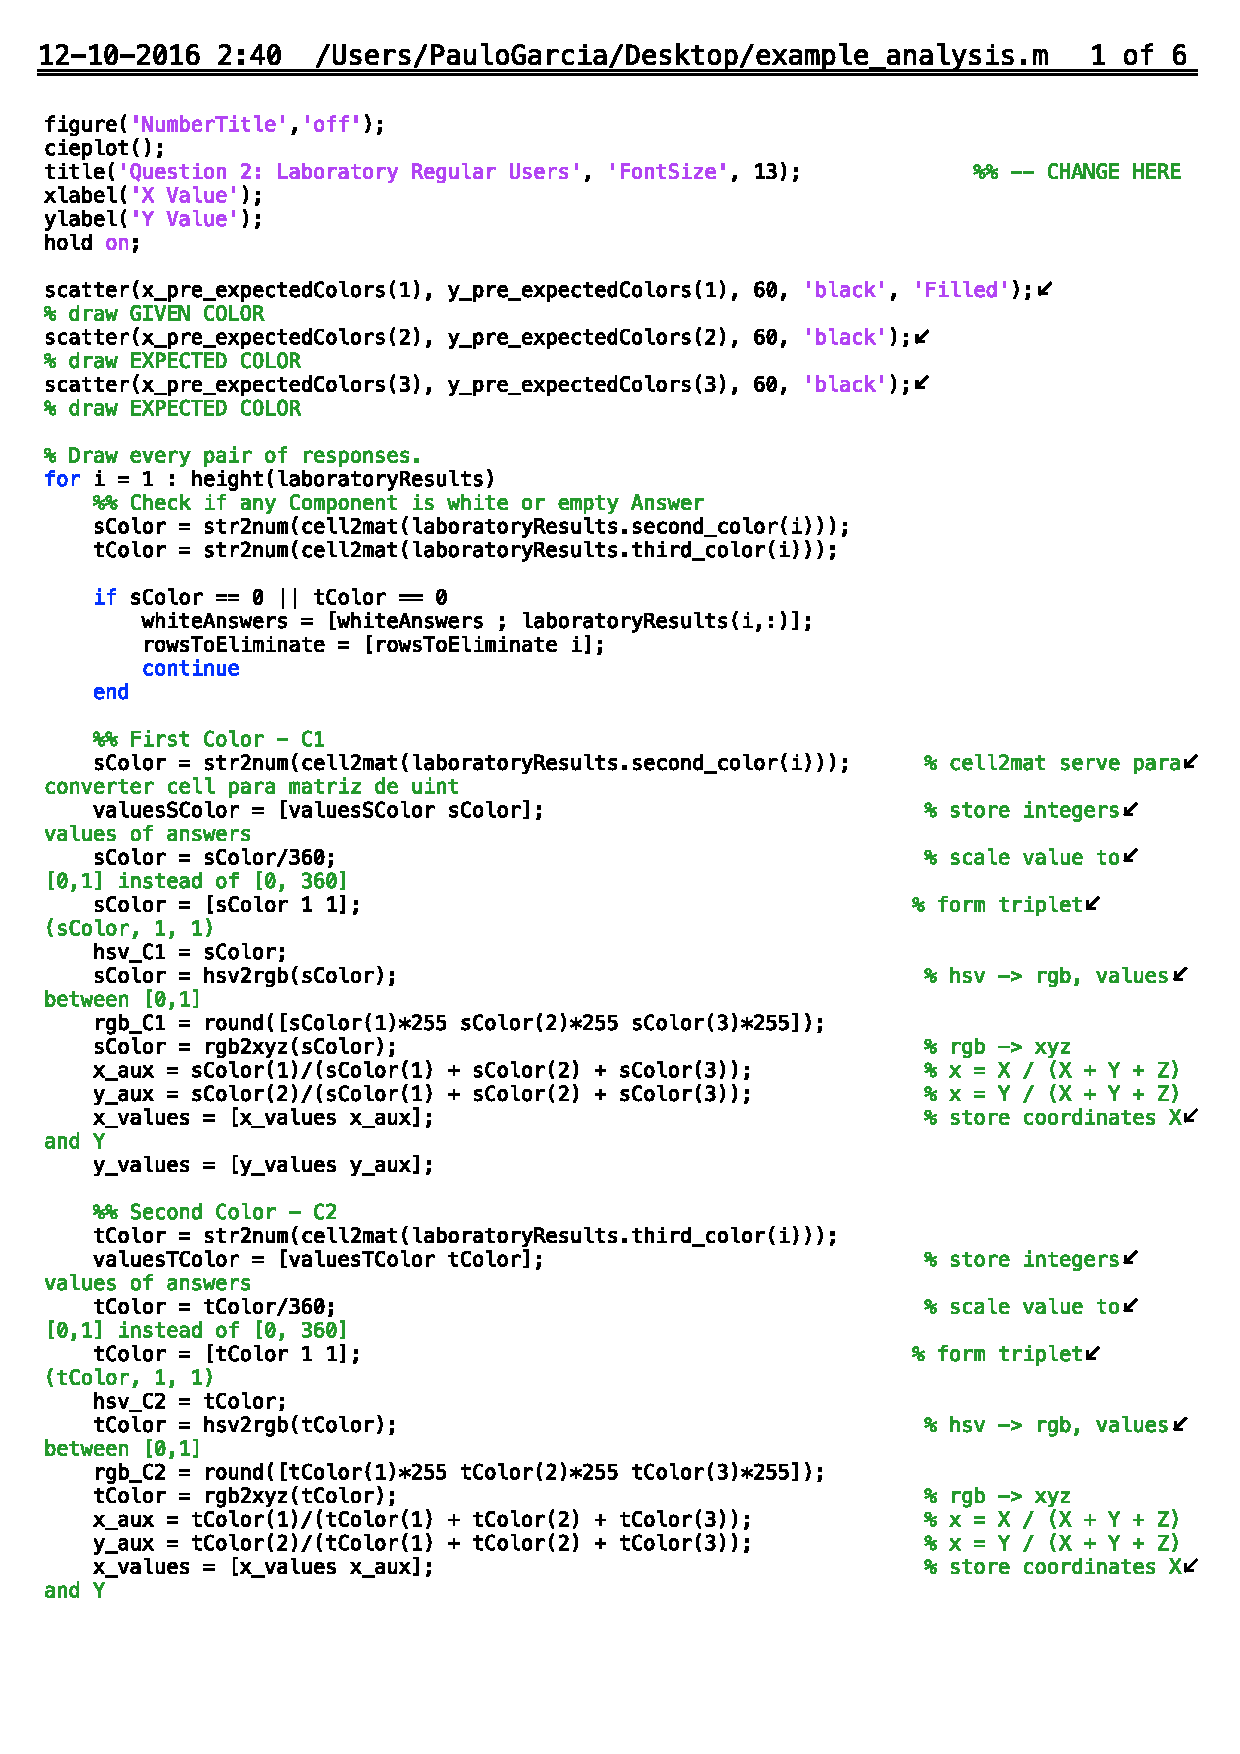
\includepdf[pages=-,pagecommand={},scale=0.88]{images/appendixes/example_analysis.pdf}

%%!TEX root = ../dissertation.tex

%%!TEX root = ../dissertation.tex

\chapter{Exercises}
\label{appendix:exercises}

Include Relevant Tables here.



% Bibliography
% Necessary for TOC to reference correctly the bibliography page
\cleardoublepage
\phantomsection
\addcontentsline{toc}{chapter}{Bibliography}
\bibliographystyle{alpha}
\bibliography{IEEEabrv,bibliography/dissertation}

% Appendix
\appendix
%!TEX root = ../dissertation.tex

% Appendix chapters entry point
% Include the chapters below

%!TEX root = ../dissertation.tex

\chapter{User Study Protocol}
\label{appendix:protocol}

\section{Motivation}
%
By conducting this first study, we intend to:
%
\begin{itemize}
  \item Conclude if there is any chance that cultural behaviours influence the user's color perception.
  \item Realize which color mixtures are more easily perceived by humans.
  \item Understand if, by using color, it is possible to clearly and easily convey information.
  This can be particularly interesting and useful when visualizing graphs or maps.
  \item Conclude if a person is capable of, not only building a mental color mixture model, but
  also deconstructing mixtures into their basic components.
\end{itemize}
%
\section{User Profiling Phase}
%
This study is anonymous and should take you up to 15 minutes. Please, answer the following answers accordingly.
%
\section{Testing Calibration Phase}
%
In this step, it's going to be presented to you a set of images. You should tune you screen definitions, in
order to answer the questions, keeping them until the end of this study. \par
%
Please, follow the steps below indicated and answer the questions.
%
\begin{enumerate}
  \item If possible, adjust your room lights for a comfortable usage of your device.
  \item Avoid reflections on your screen, by diverting the screen from direct sources of light. This step is important,
  since light reflections can affect visualization of images.
  \item To adjust the \textbf{Black Point} of your screen, define the \ul{Contrast} and \ul{Brightness} of your screen to their maximum.
  \item After Step 3, gradually reduce \textbf{Brightness} value of your screen, in order to correctly distinguish the squares of each image below [calibration squares images].
  \item If possible, define the \textbf{Color Temperature} of your screen to 6500 Kelvin Degrees.
  \item You are now ready to answer the following questions!
\end{enumerate} \par
%
\ul{NOTE:} These 6 steps are only available to the Online Users, since the Laboratory Users
do not need to perform these steps as the LCD display is already calibrated.
%
\section{Testing Color Vision Deficiences Phase}
%
This is the Color Vision Deficiencies Test. \\
%
In this step, it is going to be presented six plates with a colored pattern. Your job is to
identify the number present in each plate, typing it down in the text box below. According
to your answer, this test will inform us if you have any type of color vision deficiency which
may undermine the job of color detection. \\
%
\section{Core Test Phase}
%
Choose the Resulting color which you believe it is the result of mixing the First and Second color, by adjusting the slider below the Resulting color. \\
%
Choose two colors with which you can achieve the Resulting color, by adjusting the sliders below each color. \par
%
\ul{NOTE:} These instructions appear alternately, depending on the type of question which is shown.
%

%!TEX root = ../dissertation.tex

\chapter{Processing Data}
\label{appendix:matlab_example}
%
In this Appendix, it is available a portion of the \emph{Matlab} script which analyzed each question. Particularly, this
section analyzes the Laboratory Regular users from Question 2, which concerns the blending of Red and Blue producing Magenta. \\
%
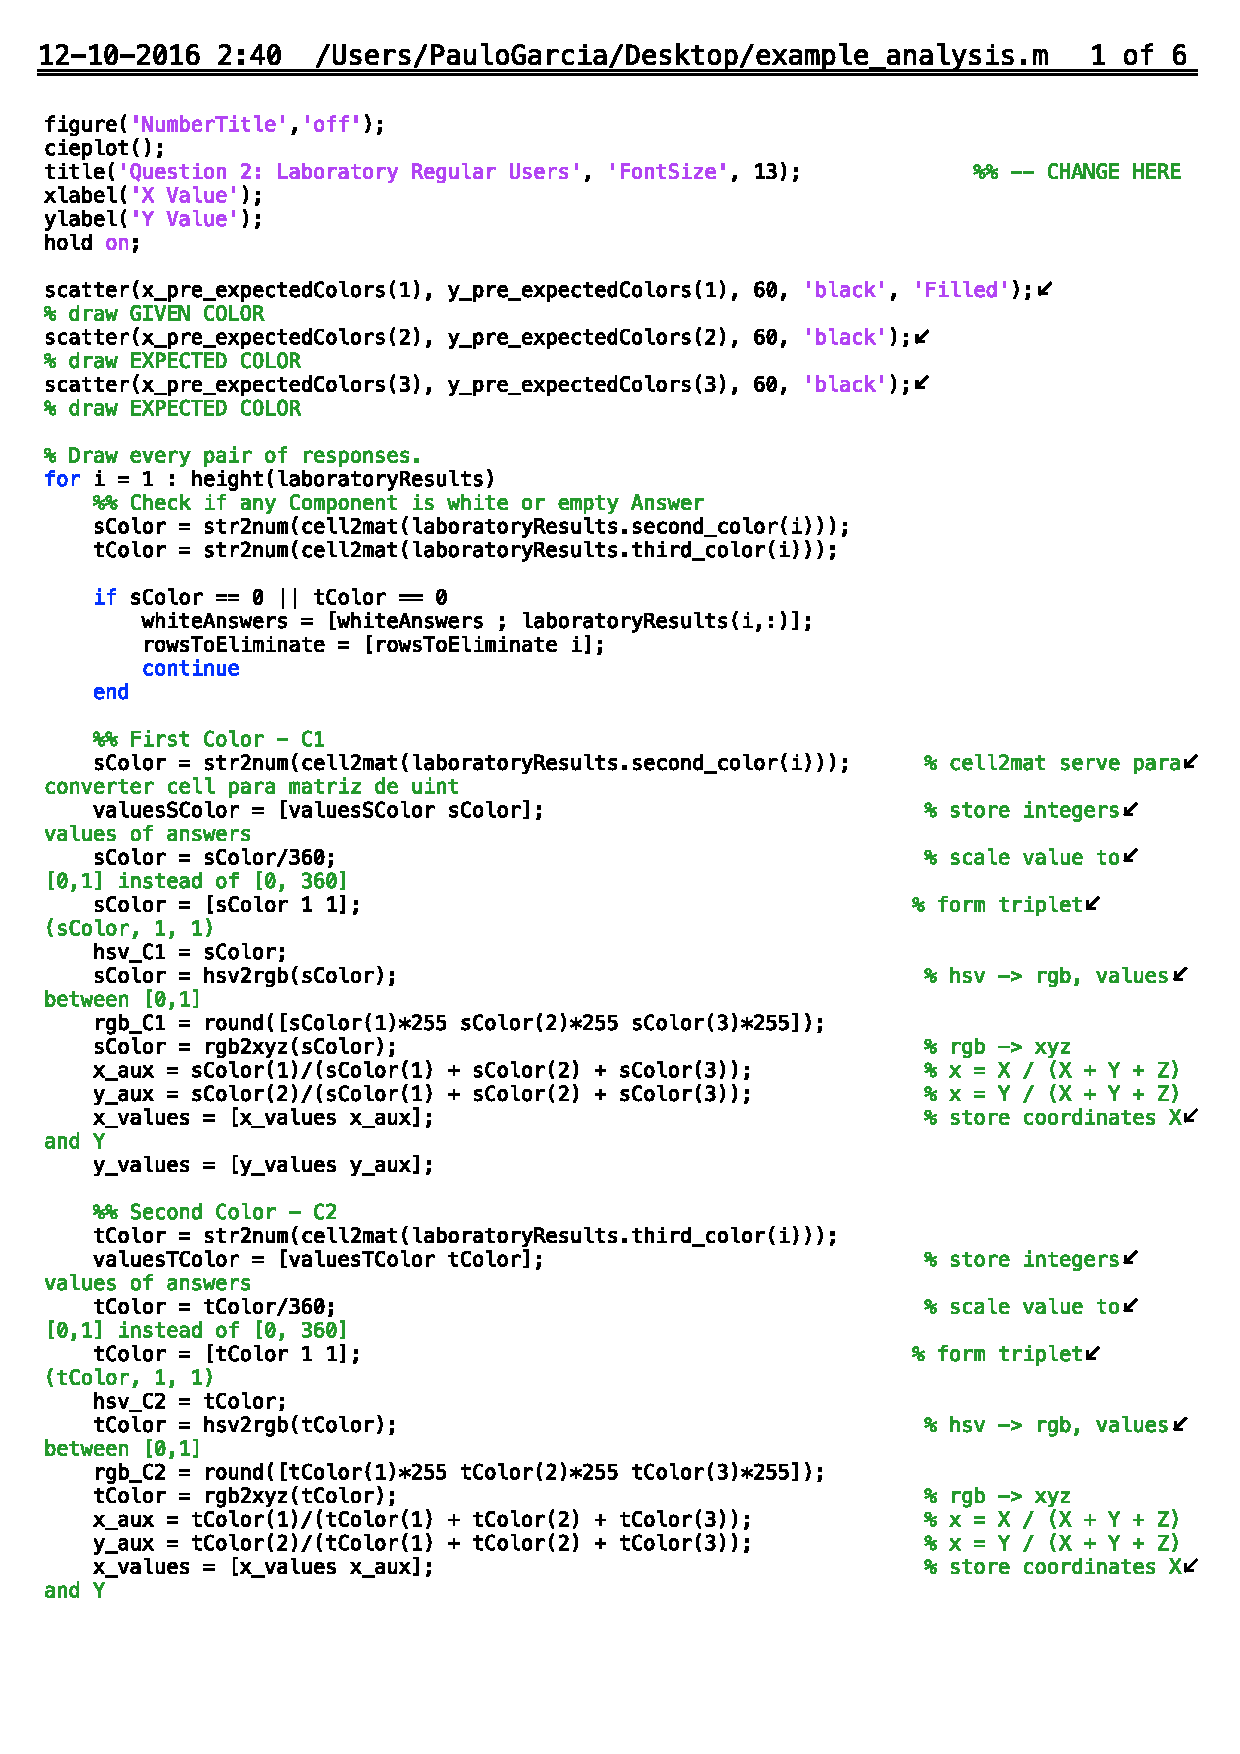
\includepdf[pages=-,pagecommand={},scale=0.88]{images/appendixes/example_analysis.pdf}

%%!TEX root = ../dissertation.tex

%%!TEX root = ../dissertation.tex

\chapter{Exercises}
\label{appendix:exercises}

Include Relevant Tables here.



\end{document}
